\documentclass[10pt,a4paper]{article}
\usepackage[utf8]{inputenc}
\usepackage[spanish]{babel}
\usepackage{a4wide}
\usepackage[sinEntregas]{caratula}
\usepackage[norelsize]{algorithm2e}
\usepackage{amsmath}
\usepackage{amssymb}
\usepackage{marginnote}
\usepackage{fancyhdr}
\usepackage{lastpage}
\usepackage{amsthm}
\usepackage{verbatim}
\usepackage{color, colortbl}
\usepackage{float}
\definecolor{Gray}{gray}{0.9}
\usepackage{tikz}
\usepackage{array}
\usepackage{amssymb}
\usepackage{graphicx}
\usepackage{subcaption}
\definecolor{gogetit}{HTML}{6C8B9F}
\definecolor{greencomments}{rgb}{0,0.5,0}

\pagestyle{fancy}
\thispagestyle{fancy}
\addtolength{\headheight}{1pt}
\lhead{Bases de Datos}
\rhead{TP1}
\cfoot{\thepage /\pageref{LastPage}}
\renewcommand{\thesubsubsection}{\thesubsection.\alph{subsubsection}}

\title{Bases de Datos - TP 1}
\author{Bases de Datos, DC, UBA.}

\begin{document}

\fecha{17 de Abril de 2015}

\materia{Bases de Datos}
%\submateria{Trabajo Pr\'actico Nº1}
\titulo{Trabajo Práctico Nº1}

\integrante{Allocati, Federico}{682/11}{fede.allocati@gmail.com}
\integrante{Izcovich, Sabrina}{550/11}{sizcovich@gmail.com}
\integrante{Pernigotti, Santiago}{870/11}{spernigotti@hotmail.com}
\integrante{Romano, Germán}{786/11}{romano.german@live.com.ar}

\maketitle

\tableofcontents

\newpage

\section{Introducción}

En el siguiente trabajo práctico, debimos diseñar e implementar una solución a un problema del mundo real utilizando herramientas de algún motor de base de datos relacional, en nuestro caso, \textit{SQLServer}.\\
\\
El problema a resolver consiste en la creación de un \textbf{Sistema de voto electrónico}. Para éste, debimos considerar que las votaciones se realizan en diferentes centros de votación que poseen mesas electorales compuestas por un presidente de mesa y su vicepresidente (o suplente). Por otro lado, pueden agregarse fiscales de cada partido político a la mesa que sirven para corroborar que el procedimiento se lleve correctamente a cabo.\\ Además, se agrega un técnico responsable de la máquina de votación, provista por el sistema. Por último, se agregan diferentes camionetas a los centros por si hay que cambiar o reparar alguna máquina. Para esto, se debe saber quién está asignado a cada una de ellas para lograr un control de las mismas.\\

El sistema debe asegurar lo siguiente:
\begin{itemize}
\item Se abarca todo el territorio de la nación y se soportan elecciones de cualquier cargo público de cada territorio que la compone. 
\item Se proveen los candidatos de cada elección y su partido político, como también la posibilidad de soportar varias elecciones desde el momento que se implemente.
\item Se soportan consultas populares hacia la ciudadanía.
\item Se respeta la confidencialidad de la elección del ciudadano.
\item Se guarda internamente el padrón electoral, esto es, en qué mesa vota cada ciudadano.
\item Se provee para cada mesa una máquina donde cada ciudadano puede elegir su opción.
\end{itemize}

Para lograr esto, debimos realizar un \textbf{Modelo de Entidad Relación} y su \textbf{Modelo Relacional} derivado. Luego, fue necesario diseñar la solución de forma física implementada en el motor de base de datos elegido. Por otro lado, realizamos el código correspondiente a las consultas/stored procedures/triggers pedidos. Finalmente, desarrollamos nuestros propios tests correspondientes a las funcionalidades de la API y extrajimos las conclusiones de la integralidad del trabajo práctico.

\newpage
\section{Modelo de Entidad Relación}

\begin{figure}[H] %[h] Aqui [b] para button [t] para top
\begin{center}
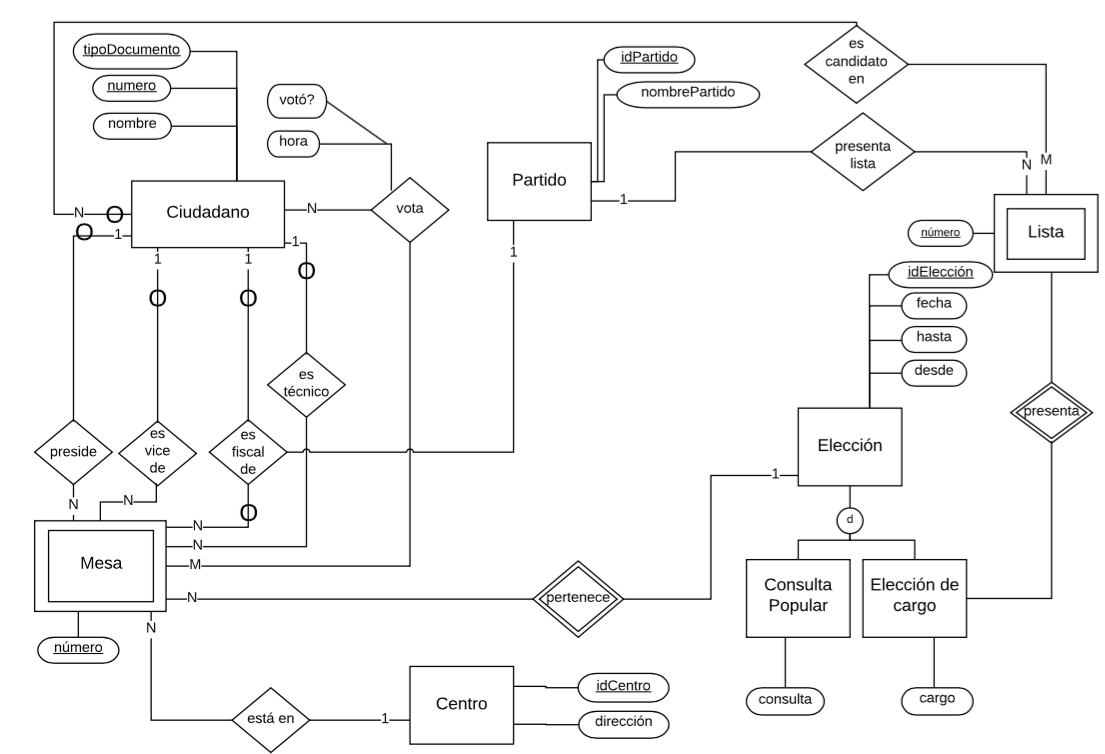
\includegraphics[width=450pt]{./diagramas/DER01.png}
\end{center}
\end{figure}

\begin{figure}[H] %[h] Aqui [b] para button [t] para top
\begin{center}
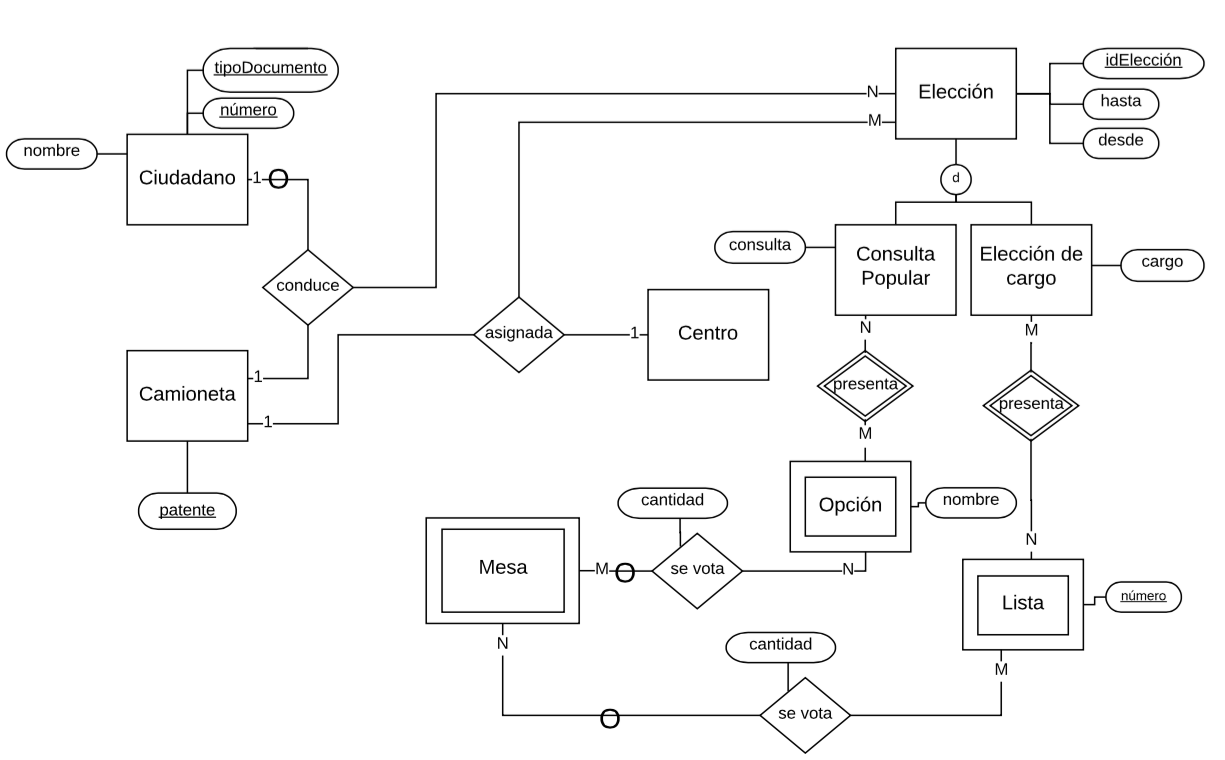
\includegraphics[width=450pt]{./diagramas/DER02.png}
\end{center}
\end{figure}

\subsection{Restricciones}
Presentamos las restricciones del Diagrama en lenguaje natural:
\begin{itemize}
\item Un ciudadano puede: presidir una mesa, o ser vicepresidente, o fiscal, o técnico, o chofer de camioneta, o ninguna de las anteriores. No puede desempeñar más de uno de los roles mencionados en una elección.
\item En una mesa se puede votar por una lista sólo si esa mesa pertenece a una elección de cargo.
\item En una mesa se puede votar por una opción (sí/no) sólo si esa mesa pertenece a una consulta popular.
\item Un ciudadano puede votar sólo en la mesa que le fue asignada en el padrón electoral.
\item Un candidato no puede figurar en dos listas distintas en una elección.
\item Un ciudadano no puede votar dos veces en una misma elección.
\item Un ciudadano puede presidir, vice-presidir, fiscalizar o ser el técnico encargado de hasta una mesa por elección.
\item Una camioneta puede estar asignada a un sólo centro.
\item En una mesa o bien se votan lista, o bien se votan opciones, según el tipo de elección en la que participe.
\item La camioneta que conduce un ciudadano para una elección debe estar asignada a esa misma elección.
\item Si un centro está asignado a una elección entonces ese centro tiene al menos una mesa que pertenece a esa elección.

\end{itemize}
\newpage
\section{Modelo Relacional}

\newpage
\section{Supuestos asumidos}
Para un correcto diseño del Sistema, debimos tomar las siguientes decisiones sobre la situación presentada:
\begin{itemize}
\item Consideramos que los ciudadanos que están en el padrón se encuentran habilitados para votar.
\item Las elecciones no duran más de un día.
\item En una consulta popular, se puede optar por Sí o por No.
\end{itemize}
%\newpage


%\section{Diseño físico}

%\newpage
%\section{Consultas, Stored Procedures y Triggers}

%\newpage
%\section{Tests}

%\newpage
%\section{Conclusiones}

\end{document}